\documentclass[12pt,prb,aps,epsf]{article}
\usepackage[utf8]{inputenc}
\usepackage{amsmath}
\usepackage{amsfonts}
\usepackage{amssymb}
\usepackage{graphicx} 
\usepackage{latexsym} 
\usepackage[toc,page]{appendix}
\usepackage{listings}
\usepackage{xcolor}
\usepackage{soul}
\usepackage[T1]{fontenc}
\usepackage{amsthm}
\usepackage{mathtools}
\usepackage{setspace}
\usepackage{array,multirow,makecell}
\usepackage{geometry}
\usepackage{textcomp}
\usepackage{float}
%\usepackage{siunitx}
\usepackage{cancel}
%\usepackage{tikz}
%\usetikzlibrary{calc, shapes, backgrounds, arrows, decorations.pathmorphing, positioning, fit, petri, tikzmark}
\usepackage{here}
\usepackage{titlesec}
%\usepackage{bm}
\usepackage{bbold}

\geometry{hmargin=2cm,vmargin=2cm}

\begin{document}
	
	\title{LP 04 Précession dans les domaines macroscopique et microscopique}
	\author{Naïmo Davier}
	
	\maketitle
	
	\tableofcontents
	
	\pagebreak
	
	
\subsection{Pré-requis}
Mécanique du point et des solides.\\
Moment cinétiques et magnétiques en mécanique quantique.

\subsection{Introduction}
On va étudier au cours de cette leçon un mouvement particulier : la précession. L'exemple couramment observé est celui d'une toupie, qui bien que soumise à la gravité, ne tombe pas tant qu'elle possède une vitesse de rotation suffisamment conséquente. Cette dynamique peu intuitive en apparence se trouve assez facilement expliquée en utilisant la notion introduite précédemment de moment cinétique, comme nous allons le voir dans cette leçon.

\section{Le gyroscope}
\textbf{Pérez mécanique chapitre 26 p 435-438}\\

On va considérer le cas ici d'un solide $\mathcal{S}$ possédant un point fixe dans le référentiel du laboratoire, pris comme étant galiléen. Ce solide a donc trois degrés de liberté de rotation et on pourra ainsi décrire son mouvement à partir des angles d'Euler.\\

\begin{figure}[h]
	\centerline{\includegraphics[width=8cm]{euler}}
\end{figure}

Prenons maintenant le cas du gyroscope qui vérifie cette condition pour son centre de masse $C$ (alors confondu avec l'origine O par la suite) grâce à une suspension constituée de trois liaisons pivots indépendantes comme présenté sur la figure suivante\\

\begin{figure}[h]
	\centerline{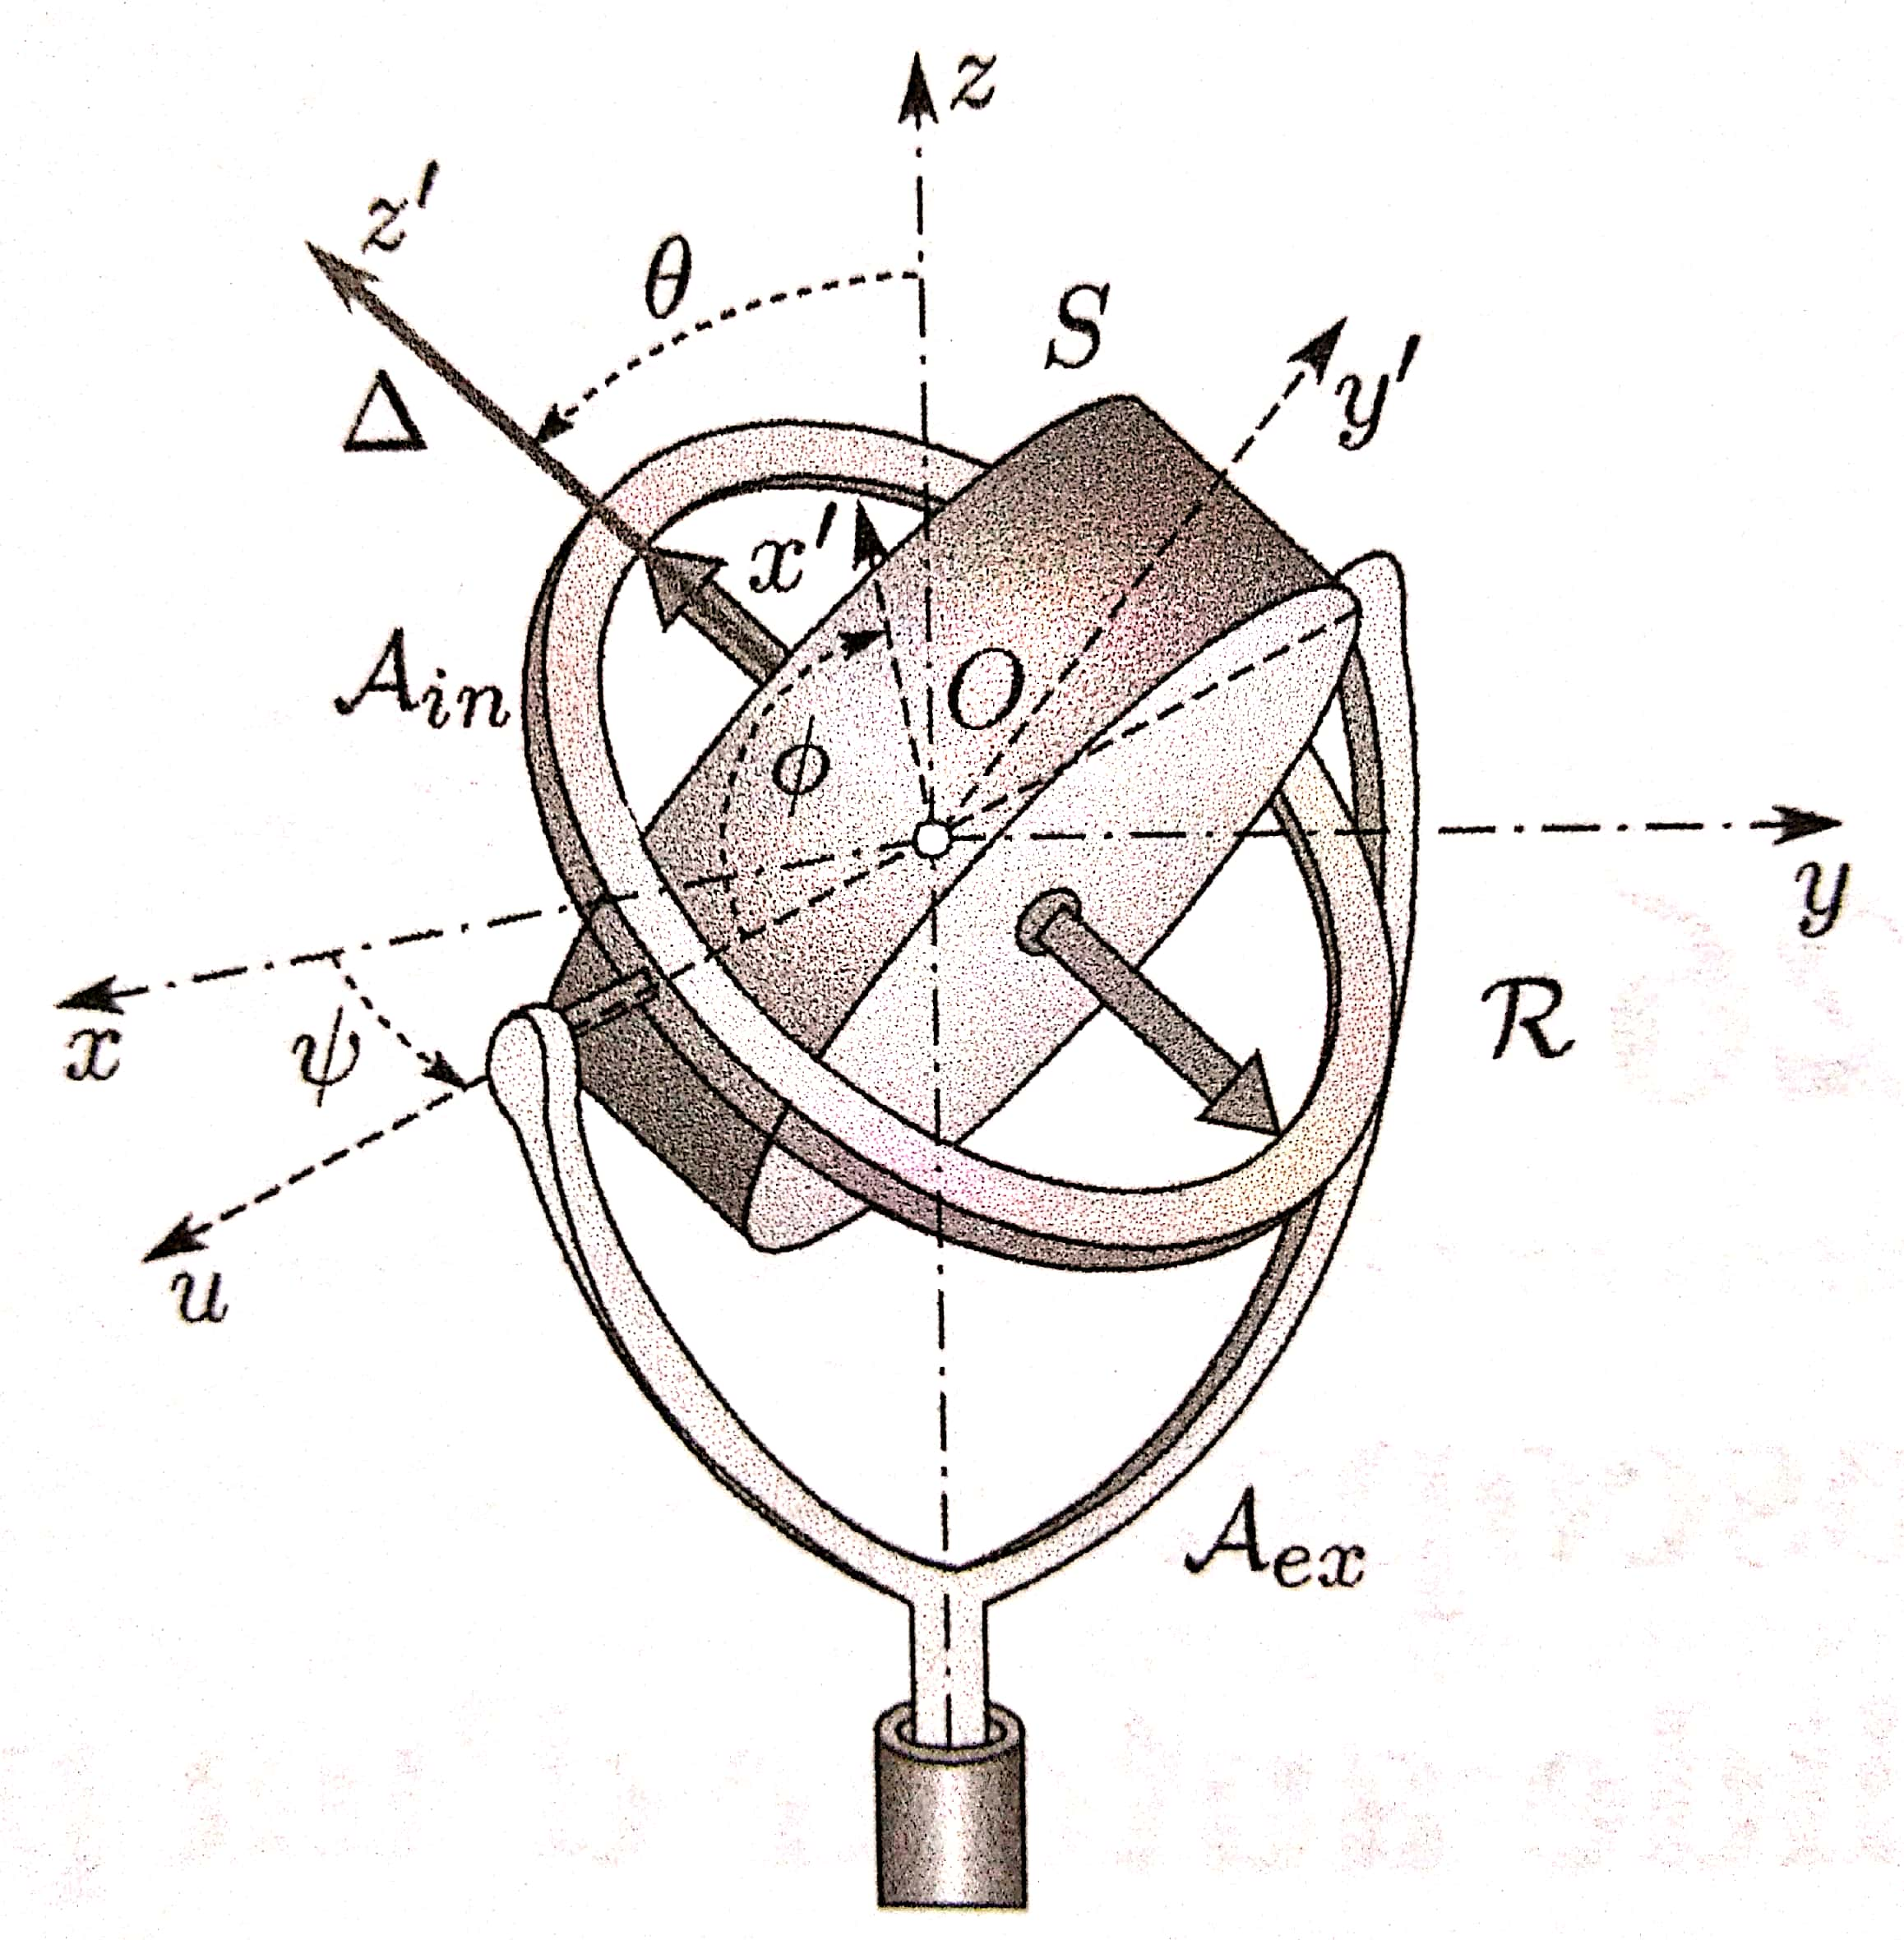
\includegraphics[width=10cm]{gyroscope}}
\end{figure}

Si les trois liaisons pivot son parfaite, c'est à dire qu'il n'y a aucuns frottements, on a que le moment des actions de contact en O, $\vec{\Gamma}_o$, est nul, puisque la puissance des actions de contact 
\begin{eqnarray}
\mathcal{P}_o = \vec{R}.\vec{v}_o + \vec{\Gamma_o}.\vec{\Omega}
\end{eqnarray}
(avec $\vec{R}$ la résultante des forces au point O, et $\vec{\Gamma_o}$ le moment des forces aux même point) au point O étant alors nulle, et ce pour tout $\vec{\Omega}$, on a nécessairement $\vec{\Gamma_O} = \vec{0}$.\\

On en déduit alors que 
\begin{eqnarray}
\frac{d\vec{L}_o}{dt} = \vec{0}
\end{eqnarray}
par application du théorème du moment cinétique. Cela signifie que le vecteur moment cinétique pointe toujours dans la même direction et en conservant sa norme de surcroit.
De plus, ici on a $\vec{\Omega} = \Omega\vec{e}_{z'}$ et donc $\vec{L}_o \propto \vec{\Omega}$, ce qui implique alors $ \vec{\Omega} = \vec{cste}$ aussi.\\

L'application originelle et qui semble peut être la plus évidente est que l'on peut s'en servir pour vérifier si le référentiel attaché au support sur lequel repose le gyroscope est galiléen ou non, puisque $\vec{\Omega}$ est constant uniquement par rapports aux référentiels galiléens. Ainsi si l'on place le gyroscope sur notre bureau et que l'on est assez patients on peut percevoir la rotation de la terre sur elle même, puisqu'on va voir l'axe du gyroscope tourner dans le référentiel attaché au sol.\\

On peut remarquer un fait intéressant ici : si on applique une force en un point A alors on constate grâce au théorème du moment cinétique 
\begin{eqnarray}
\frac{d\vec{L}_o}{dt}  = \vec{OA}\times \vec{F}_A
\end{eqnarray}
que l'axe de rotation sera déplacé dans la direction orthogonale au plan formé par $\vec{OA}$ et $\vec{F}_A$. Ainsi si la force est verticale le vecteur portant la direction de l'axe sera déplacé horizontalement et inversement, ce qui semble à première vue très contre intuitif puisque contraire au cas de l'action d'une force sur un point excentré d'une barre par exemple.

\subsubsection{Quelques applications}
Dans la pratique, à cause des frottements $\vec{\Omega}$ finit par s'aligner selon l'axe de la terre. Le plan vertical contenant $\vec{\Omega}$ est alors le plan méridien, et on peut déterminer sa latitude en imposant à l'axe du gyroscope de se mouvoir dans un plan horizontal, auquel cas $\vec{\Omega}$ s'orientera selon l'axe $\Delta_m$ du méridien, l'angle $(\vec{\Omega}_T,\Delta_m)$ nous donne alors la latitude.

\begin{figure}[h]
	\centerline{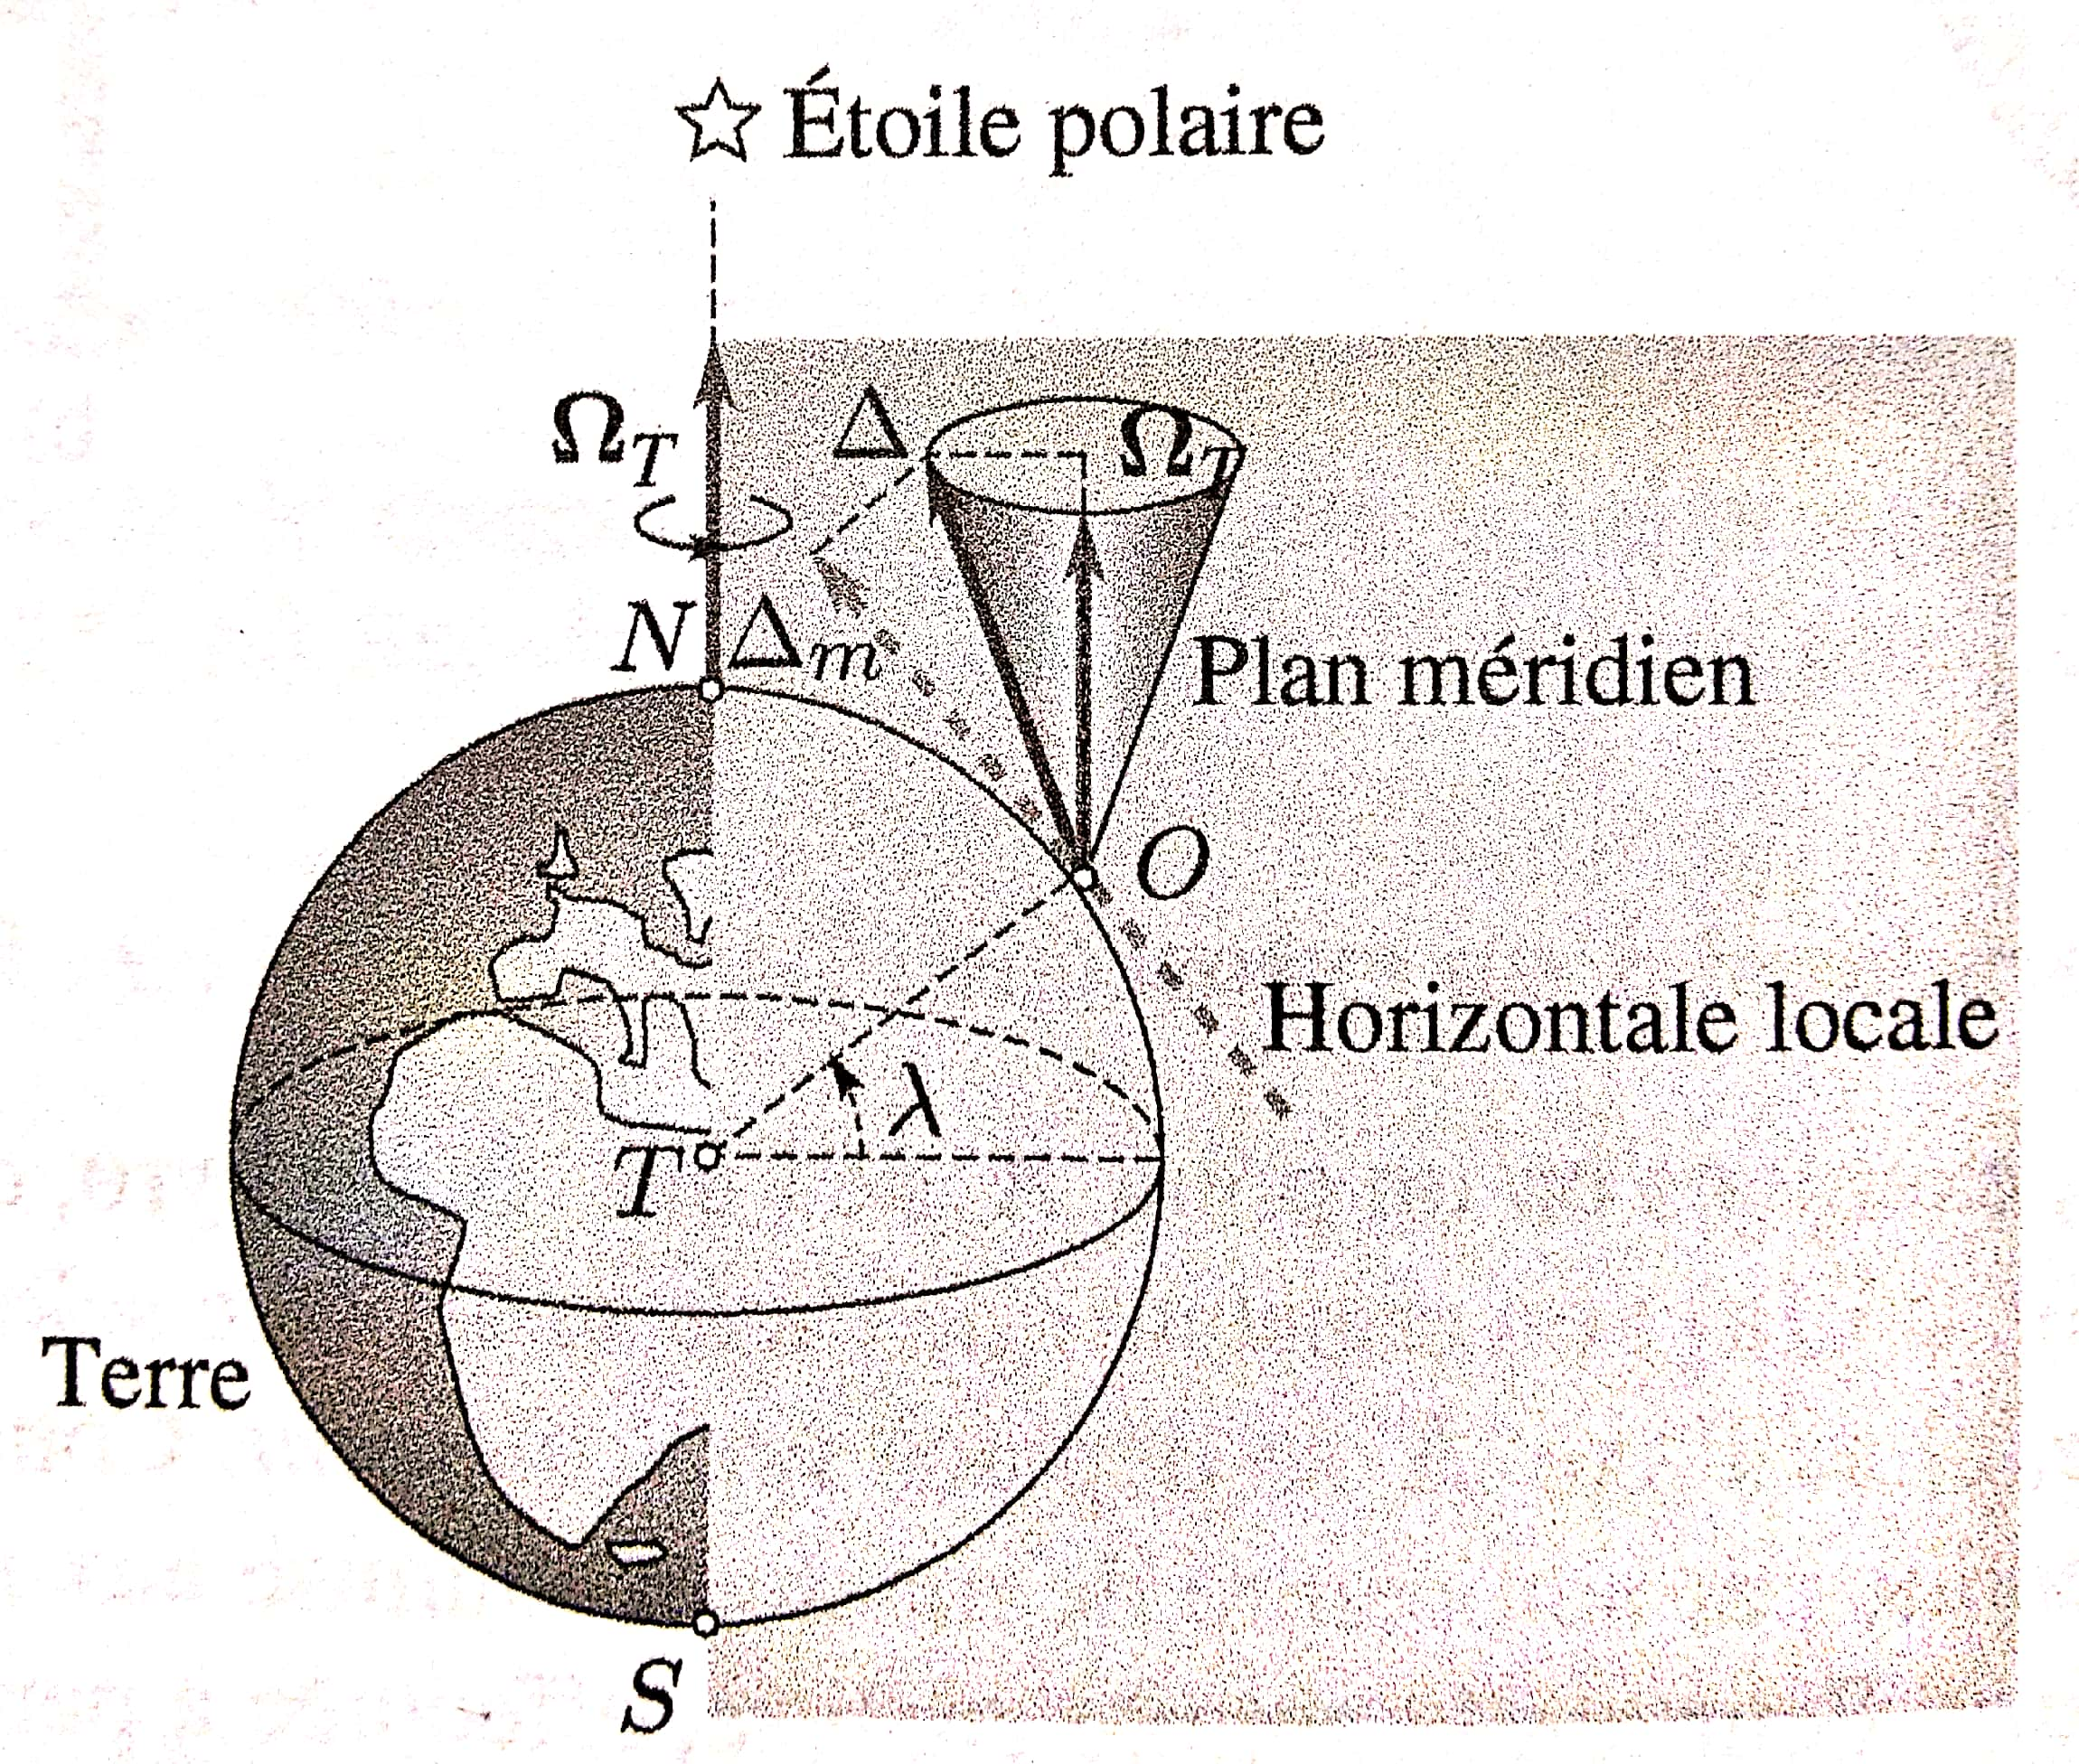
\includegraphics[width=10cm]{compas}}
\end{figure}

On peut se servir d'un gyroscope pour rectifier la trajectoire d'un avion ou d'une fusée en détectant une modification de la direction de son axe de rotation.


\section{Approximation gyroscopique et toupie}
\textbf{J.Boutigny Mécanique 2, p 179-181} pour les calculs.\\
\textbf{Pérez mécanique p 440} pour l'obtention de l'équation de précession.\\

On peut maintenant appliquer la logique introduite pour traiter le cas d'un objet commun dont la physique n'est pas triviale : la toupie. Dans la pratique on sait qu'après avoir été lancée cette dernière est capable de rester droite alors que pourtant la gravité, seule force en jeu si on oublie les frottements, tendrait à la faire chuter. Nous allons maintenant tenter de voir si 'on peut retrouver analytiquement son comportement.\\

On va à nouveau décrire le mouvement avec les angles d'Euler, tout indiqués pour ce problème. On a alors
\begin{eqnarray}
\vec{\Omega} &=& \dot{\psi} \vec{e}_z + \dot{\theta} \vec{e}_u + \dot{\phi} \vec{e}_{z'} \\
&=& \dot{\theta} \vec{e}_u + \dot{\psi}\sin{\theta}\, \vec{e}_w + (\dot{\phi} + \dot{\psi}\cos{\theta} ) \vec{e}_{z'}
\end{eqnarray}
De plus, puisque la toupie est un solide de révolution, sa matrice d'inertie est diagonale dans la base $(u ,w ,z')$ et on peut ainsi écrire 
\begin{eqnarray}
\vec{L}_o = 
\begin{pmatrix}
I & 0 & 0\\
0 & I & 0\\
0 & 0 & J
\end{pmatrix}
\begin{pmatrix}
\dot{\theta}\\
\dot{\psi} \sin \theta\\
\dot{\phi} + \dot{\psi} \cos \theta
\end{pmatrix}
 = I\dot{\theta} \vec{e}_u + I\dot{\psi}\sin{\theta}\, \vec{e}_w + J(\dot{\phi} + \dot{\psi}\cos{\theta} ) \vec{e}_{z'}
\end{eqnarray}
On peut maintenant appliquer le théorème du moment cinétique en O, sachant que le seul moment qui va entrer en compte va être celui du poids
\begin{eqnarray}
\frac{d\vec{L}_o}{dt} = \vec{OG}\times m\vec{g} = a \vec{e}_{z'}\times -mg\vec{e}_z =  mga\sin{\theta}\;\vec{e}_u \label{eq1}
\end{eqnarray}
où a est la distance de O au centre de masse.\\

On voit ici que l'équation (\ref{eq1}) est compliquée à résoudre, c'est pourquoi on peut utiliser ici l'approximation gyroscopique pour se faire assez facilement une idée du mouvement.\\
L'approximation gyroscopique consiste à estimer que la rotation autour d'un des trois axes se fait beaucoup plus rapidement que les autres. Ici en l'occurrence cela va revenir à estimer que l'on a 
\begin{eqnarray}
\dot{\phi} \gg \dot{\psi}\hspace{0.5cm}\mathrm{et} \hspace{0.5cm} \dot{\phi} \gg \dot{\theta}
\end{eqnarray} 
On aura alors 
\begin{eqnarray}
\vec{L}_o \simeq J\dot{\phi}\; \vec{e}_{z'}
\end{eqnarray}
et ainsi 
\begin{eqnarray}
\frac{d\vec{L}_o}{dt} = J\ddot{\phi}\; \vec{e}_{z'} + J\dot{\phi}\; \frac{d\vec{e}_{z'}}{dt}
\end{eqnarray}
or le vecteur $\vec{e}_{z'}$ est entrainé selon le vecteur rotation 
\begin{eqnarray}
\vec{\omega} = \dot{\theta}\vec{e}_u + \dot{\psi}\vec{e}_z = \dot{\theta}\vec{e}_u + \dot{\psi}\cos{\theta}\; \vec{e}_{z'}  + \dot{\psi}\sin{\theta}\;\vec{e}_w
\end{eqnarray}
 et on a ainsi 
\begin{eqnarray}
 \frac{d\vec{e}_{z'}}{dt} = \vec{\omega}\times \vec{e}_{z'} = -\dot{\theta}\vec{e}_w + \dot{\psi} \sin{\theta}\; \vec{e}_u
\end{eqnarray}
et finalement on obtient donc
\begin{eqnarray}
\frac{d\vec{L}_o}{dt} = J\ddot{\phi}\; \vec{e}_{z'} - J\dot{\phi} \dot{\theta}\;\vec{e}_w + J\dot{\phi}\dot{\psi} \sin{\theta}\; \vec{e}_u
\end{eqnarray}
ce qui mène, en appliquant le théorème du moment cinétique à 
\begin{eqnarray}
J\dot{\phi}\dot{\psi} \sin{\theta} &=& mga \sin\theta\\
\dot{\phi} \dot{\theta} &=& 0\\
\ddot{\phi} &=& 0
\end{eqnarray}
On a donc $\dot{\phi}= cste$, ce qui signifie que la vitesse de rotation de la toupie sur elle même est conservée. De plus on a 
\begin{eqnarray}
\dot{\psi} = \frac{mga}{J\dot{\phi}}
\end{eqnarray}
et $\theta =cste$ ce qui nous dit que le le sommet de la toupie tourne autour de l'axe $Oz$ à vitesse constante et en conservant sont inclinaison.
Ce mouvement est précisément celui que l'on nomme précession : la toupie précesse autour de l'axe $Oz$.\\

On aurait pu intuiter ce résultant en faisant directement l'approximation gyroscopique pour exprimer 
\begin{eqnarray}
\vec{OC} \simeq a\frac{\vec{L}_o}{L_o}
\end{eqnarray} 
et ainsi avoir 
\begin{eqnarray}
\frac{d\vec{L}_o}{dt} \simeq  \vec{L}_o \times \frac{m\vec{g}a}{L_o}  = \vec{\Omega}_p \times \vec{L}_o \hspace{0.4cm}\mathrm{avec}\; \vec{\Omega}_p = \frac{mga}{J\dot{\phi}}\vec{e}_z
\end{eqnarray}
ce qui est précisément l'équation d'un mouvement de précession du vecteur $\vec{L}_o$ autour de la direction portée par $\vec{\Omega}_p$ à la pulsation $\Omega_p$.

\section{Application au cas microscopique d'un moment magnétique - RMN}

\textbf{Cohen Tannoudji tome 1 complément F du chapitre IV p 459-466}\\

Un autre exemple de mouvement de précession est ce lui de la résonance magnétique, dont on a en général déjà entendu parler en chimie sans pour autant rentrer dans les détails. On va ainsi ici brièvement en expliquer le principe, en commençant par regarder le mouvement d'un spin, celui d'un proton par exemple, plongé dans un champ magnétique extérieur.

\subsection{Traitement classique}

On considère un système de moment cinétique $\vec{j}$ et de moment magnétique $\vec{m}=\gamma \vec{j}$ avec $\gamma$ le rapport gyromagnétique du système. On le plonge dans un champ magnétique $\vec{B}_0$ qui exerce alors par définition de $\vec{m}$ un couple $\vec{m}\times \vec{B}_0$ ce qui mène, par application du théorème du moment cinétique à 
\begin{eqnarray}
\frac{d\vec{j}}{dt} = \vec{m}\times \vec{B}_0 \; \Leftrightarrow \; \frac{d\vec{m}}{dt} = \gamma \vec{m}\times \vec{B}_0 \label{précess}
\end{eqnarray}
on voit que l'on obtient une équation analogue à celle de la partie précédente, nommée équation de Larmor, avec cette fois $\vec{\Omega} = -\gamma\vec{B}_0$, qui décrit donc un mouvement de précession.

On peut d'ailleurs montrer facilement que la norme de $\vec{j}$ est conservée en faisant (\ref{précess})$.\vec{j}$, et que de même (en faisant (\ref{précess})$.\vec{B}_0$) sa projection selon l'axe porté par $\vec{B}_0$ est elle aussi constante.\\

L'idée est maintenant d'ajouter au champ statique $\vec{B}_0$ un champ $\vec{B}_1(t)$, orthogonal à $\vec{B}_0$ et tournant à la vitesse angulaire $\vec{\omega}$.\\
\begin{figure}[h]
	\centerline{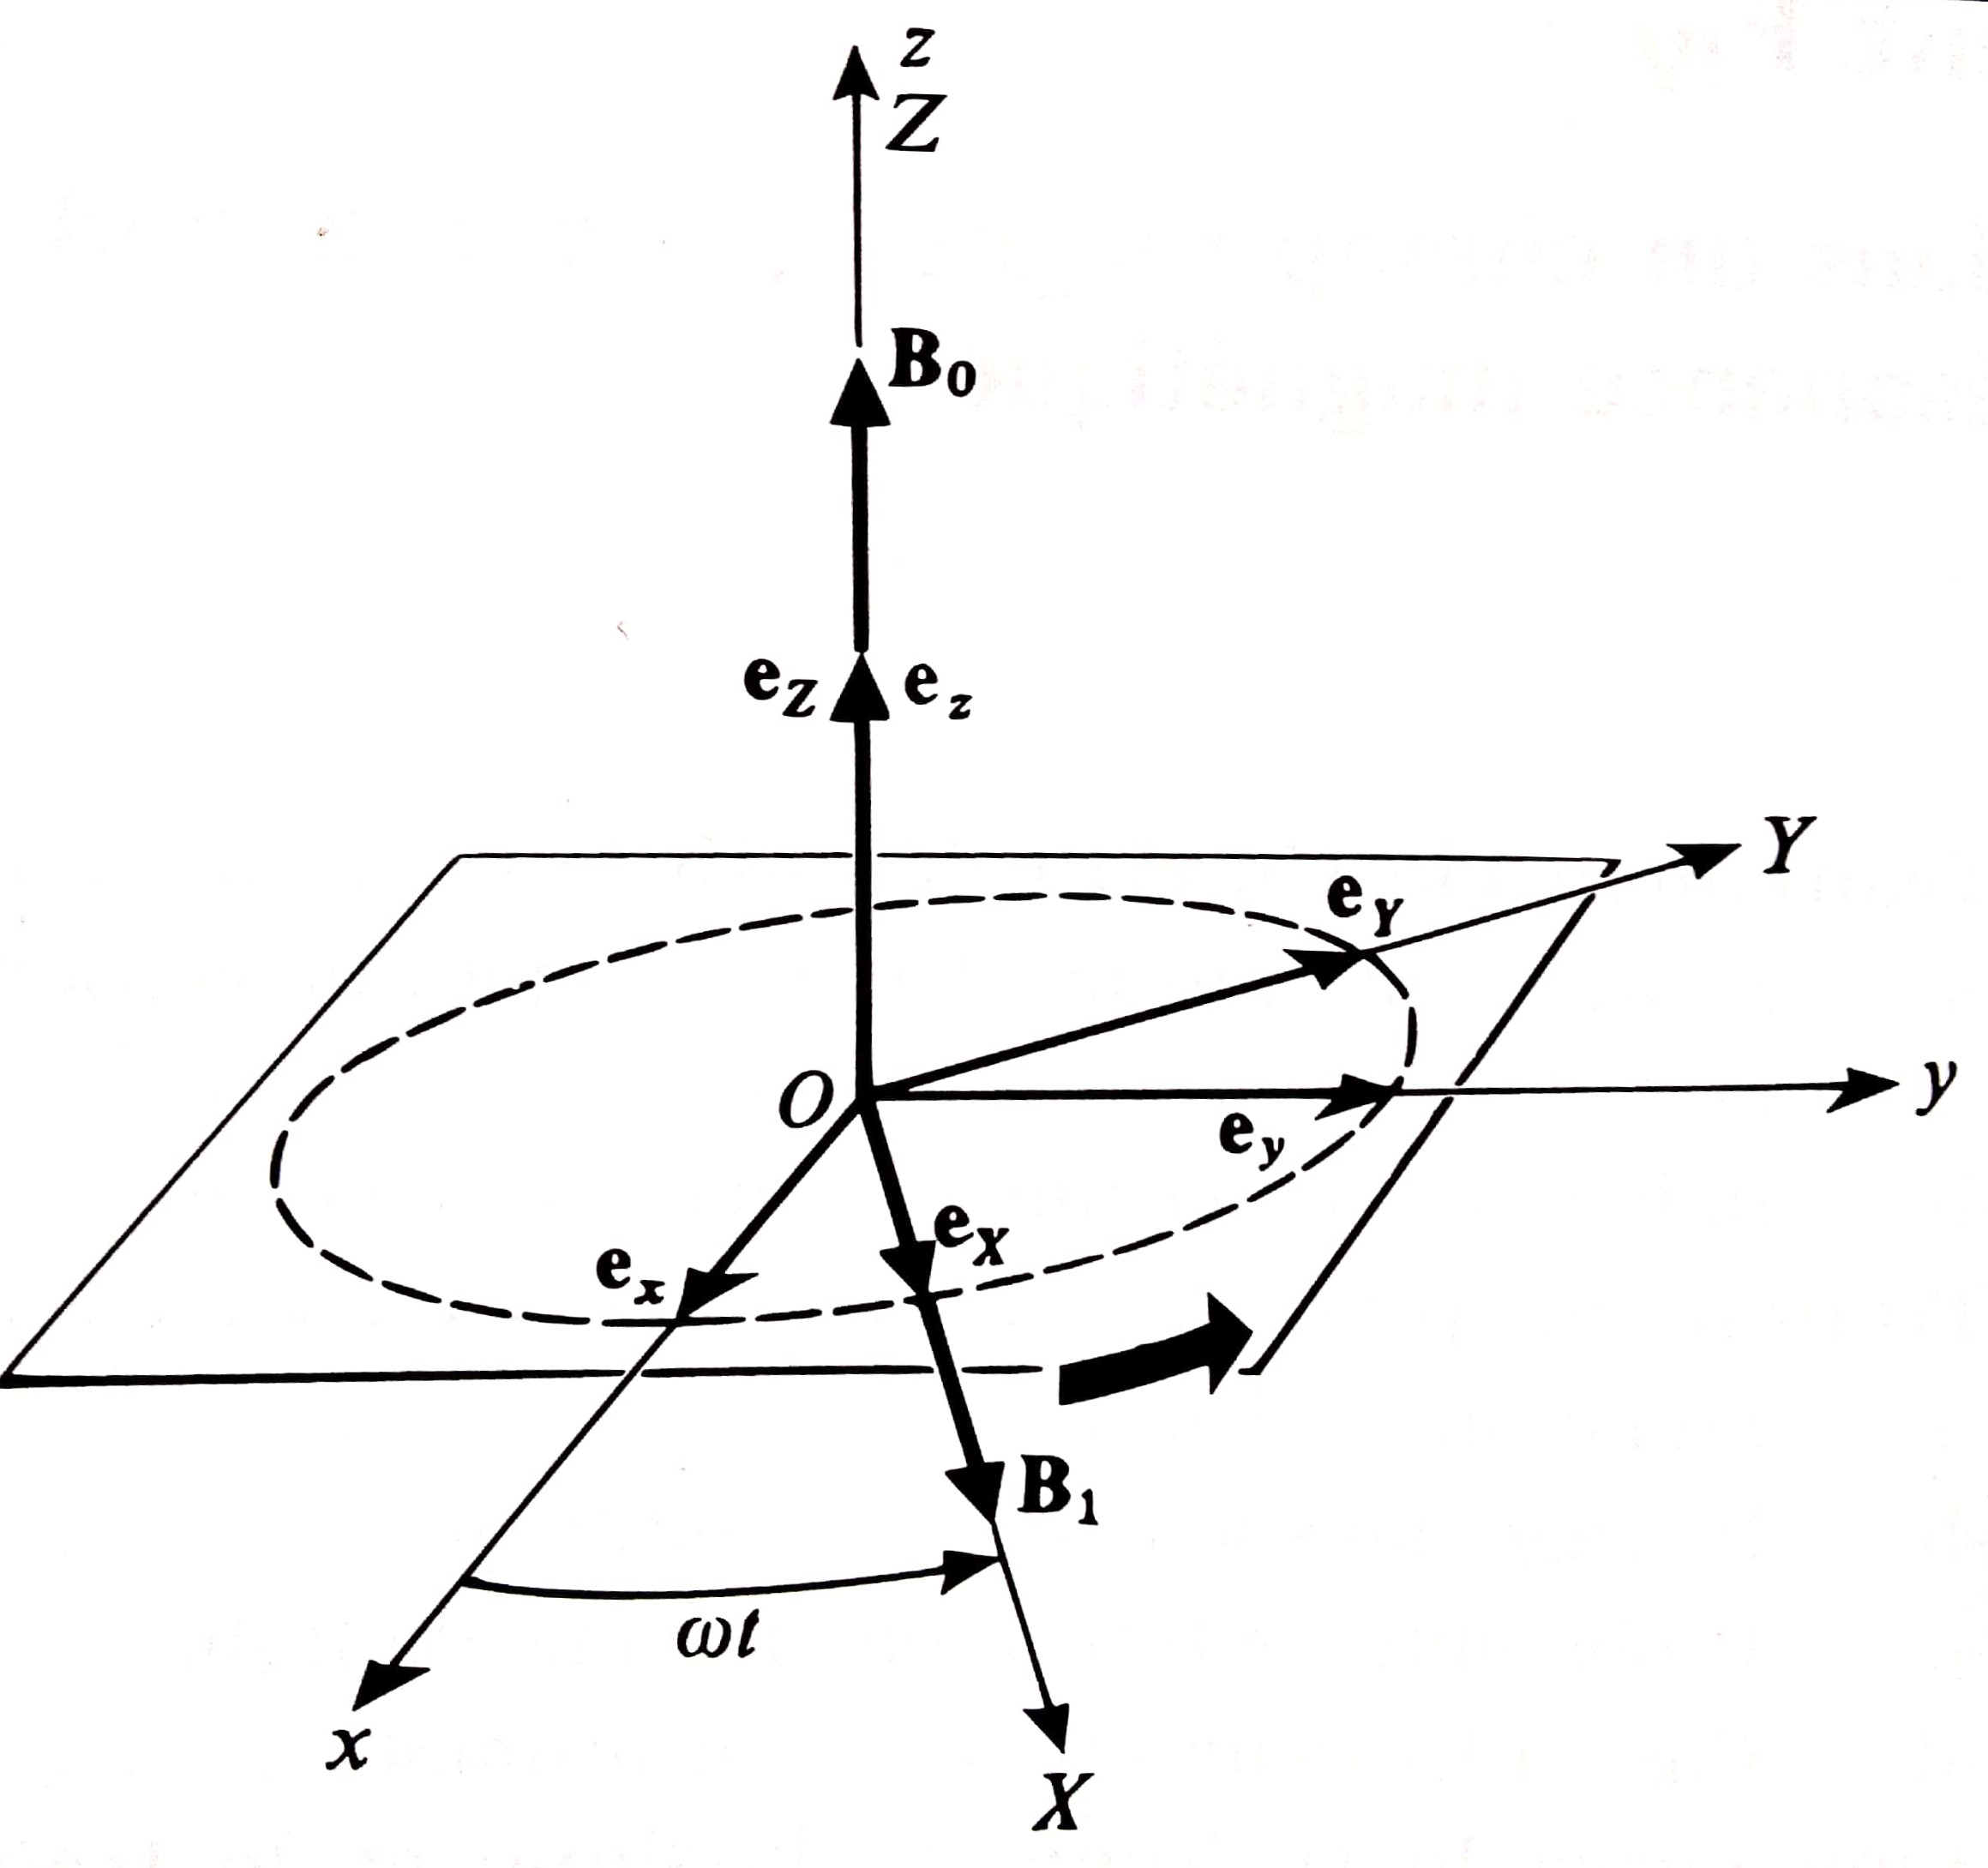
\includegraphics[width=10cm]{champs}}
\end{figure}

On a alors 
l'équation 
\begin{eqnarray}
\frac{d\vec{m}}{dt} = \gamma \vec{m}\times [\vec{B}_0 + \vec{B}_1(t)]
\end{eqnarray}
qui est pénible à résoudre car $\vec{B}_1$ dépend du temps. Il est donc plus commode de se placer dans le repère $R' = OXYZ$ porté par $\vec{B}_0$ et $\vec{B}_1$, dans lequel $\vec{m}$ a la vitesse relative
\begin{eqnarray}
\left(\frac{d\vec{m}}{dt}\right)_{R'} = \frac{d\vec{m}}{dt} - \omega \vec{e}_z \times \vec{m}
\end{eqnarray}
on  a donc : 
\begin{eqnarray}
\left(\frac{d\vec{m}}{dt}\right)_{R'} &=& \vec{m} \times [\gamma \vec{B}_0 + \gamma \vec{B}_1 + \omega \vec{e}_z]\\
&=& \vec{m} \times [\Delta \omega \,\vec{e}_Z - \omega_1 \vec{e}_X]
\end{eqnarray}
où on a posé $\omega_0 = -\gamma B_0$, $\omega_1 = -\gamma B_1$ et $\Delta\omega = \omega - \omega_0$.\\

Le second membre de cette équation est maintenant à coefficients constants, et on reconnait un mouvement de précession autour du champ 
\begin{eqnarray}
\vec{B}_{eff} = \frac{1}{\gamma} [\Delta \omega \,\vec{e}_Z - \omega_1 \vec{e}_X]
\end{eqnarray}
Pour obtenir le mouvement absolu de $\vec{m}(t)$ il suffit de composer l'expression obtenue avec une rotation autour de $Oz$ à la vitesse angulaire $\omega$.

\begin{figure}[h]
	\centerline{\includegraphics[width=8cm]{bef}}
\end{figure}

Si à l'instant initial on a $\vec{m} = m\vec{e}_z$ alors il y a deux cas limites possibles 
\begin{itemize}
	\item Soit $\Delta \omega \gg \omega_1$ et alors $\vec{m}$ reste près et précesse autour de $\vec{e}_z$.
	\item Soit $\Delta \omega \ll \omega_1$ et dans ce cas $\vec{m}$ précesse cette fois autour de $\vec{B}_1$. Lorsque $\Delta \omega = 0$ on dit alors qu'on est à la résonance magnétique, et alors $\vec{m}$ tourne dans le plan $XOZ$.
\end{itemize}

\subsection{Aspect quantique}
A ce point on peut regarder notre système du point de vue quantique. On sait que dans la configuration étudiée le spin (ou moment magnétique) considéré a deux états propres $|+\rangle$ et $|-\rangle$ selon la direction $Oz$ fixée par $\vec{B}_0$. Si on se place dans le cas résonnant $\omega = \omega_0$ on a alors $\vec{m}$ qui tourne dans le plan $OXZ$. Le hamiltonien est décrit dans ce cas par 
\begin{eqnarray}
H = -\vec{M}.\vec{B} = - \gamma \vec{S}.\vec{B}_0
\end{eqnarray}
puisque $\vec{m}$ étant dans le plan $OXZ$ on a alors $\vec{M}.\vec{B}_1 = 0$.
On a alors deux énergies propres 
\begin{eqnarray}
E_+ = -\frac{\gamma\hbar B_0}{2}\hspace{0.4cm}\mathrm{et}\hspace{0.4cm}E_- = \frac{\gamma\hbar B_0}{2}
\end{eqnarray}
et donc l'état $|+\rangle$ est l'état fondamental. On comprend alors que la précession autour de $\vec{B}_1$ (dans le plan $OXZ$) va permettre de retourner le spin et ainsi de faire passer le système de l'état $|+\rangle$ à l'état excité $|-\rangle$. Les spin qui sont dans l'état excité peuvent alors se désexciter en émettant un photon d'énergie 
\begin{eqnarray}
\Delta E = E_- - E_+ = \gamma\hbar B_0
\end{eqnarray}
On pourra ensuite, en fonction du nombre de photon détectés, et de la fréquence des photons reçus déterminer quels sont les groupes de protons équivalents dans l'échantillon étudié mais on glisse là dangereusement vers la chimie.

\section{Conclusion}
On a pu aujourd'hui mettre en œuvre les outils développés en mécanique du solide pour traiter le cas atypique du mouvement de précession. Il est de plus possible de traiter d'autres cas représentatifs de ce phénomène tels que la précession des équinoxes par exemple.

\section*{Questions}
Origine du lien entre $\vec{j}$ et $\vec{m}$.\\

Autres exemples de précession ?\\

Autre type de résonance magnétique.\\
$\rightarrow$ résonance due aux nuages électroniques ayant des moments magnétique (cf modèle de Bohr).\\

Expliquer brièvement la précession des équinoxes.

\section*{Remarques}
Montrer une toupie, un gyroscope sur un plateau tournant ou une vidéo.

\end{document}